\documentclass[main.tex]{subfiles}

\begin{document}

\begin{tikzpicture}[]

	\node at (0,0) {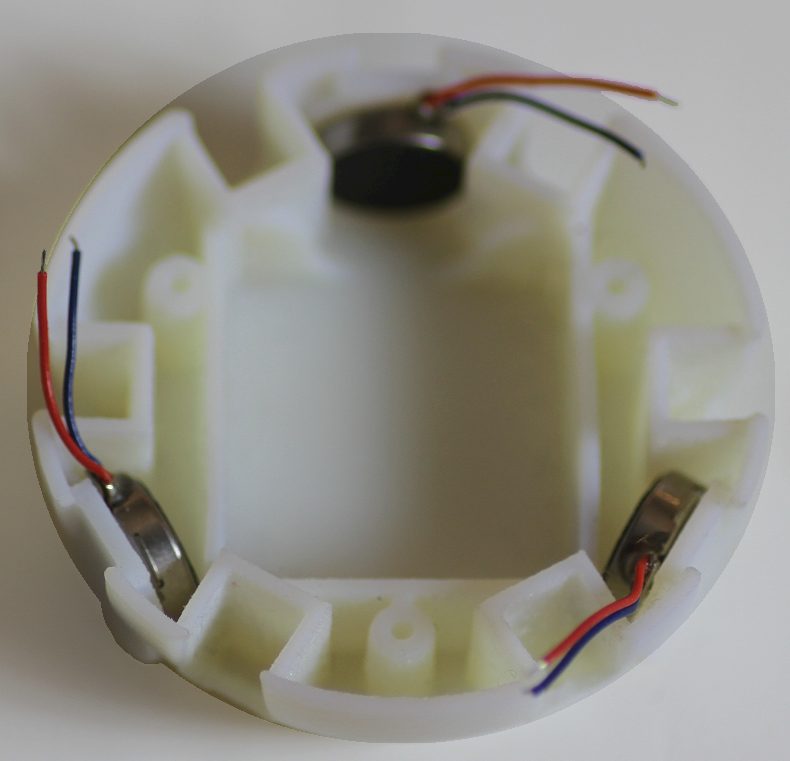
\includegraphics[scale=0.3]{Images/motorLocations2.png}};

	%\node[opacity=0.4] at (90:2.75) (m0W) {\contour{white}{\Large$m_0$}};
	%\node[] at (90:2.75) (m0) {\Large$m_0$};
	%\node[opacity=0.4] at (-30:3.25) (m1W) {\contour{white}{\Large$m_1$}};
	%\node[] at (-30:3.25) (m1) {\Large$m_1$};
	%\node[opacity=0.4] at (-145:3.25) (m2W) {\contour{white}{\Large$m_2$}};
	%\node[] at (-145:3.25) (m2) {\Large$m_2$};

	\node[] at (90:1) (m0) {\Large$m_1$};
	\node[] at (-30:1.65) (m1) {\Large$m_2$};
	\node[] at (-145:1.65) (m2) {\Large$m_3$};

	\node[] at (-88:1.2)  (l0) {\Large$l_1$};
	\draw[thick,->] (-88:1.45) -- (-88:1.85);

	\node[] at (153:1.3)  (l1) {\Large$l_2$};
	\draw[thick,->] (153:1.5) -- (153:1.85);

	\node[] at (26:1.3)  (l2) {\Large$l_3$};
	\draw[thick,->] (26:1.45) -- (26:1.90);

\end{tikzpicture}



\end{document}